\section{Question 6}

\subsection{Task}
Consider a transformation by which a function $y_i\left(x_i\right)$ is transformed to another function $m_i\left(c_i\right)$  where $m$ and $c$ are slope and intercept of the original curve at different points on the curve represented by $y$ as function of $x$. The envelope of lines of slope $m$ drawn at each value of $c$ has the same shape as that of the curve drawn using the points $\left(x,y\right)$. This is illustrated a parabola as shown in the figures below. Write a program that converts a function given as $y\left(x\right)$ to the new form either graphically or analytically. Make sure your process works even when the function $y\left(x\right)$ is changed to any other smooth and well-behaved function.
\begin{figure}[!ht]
\begin{center}
	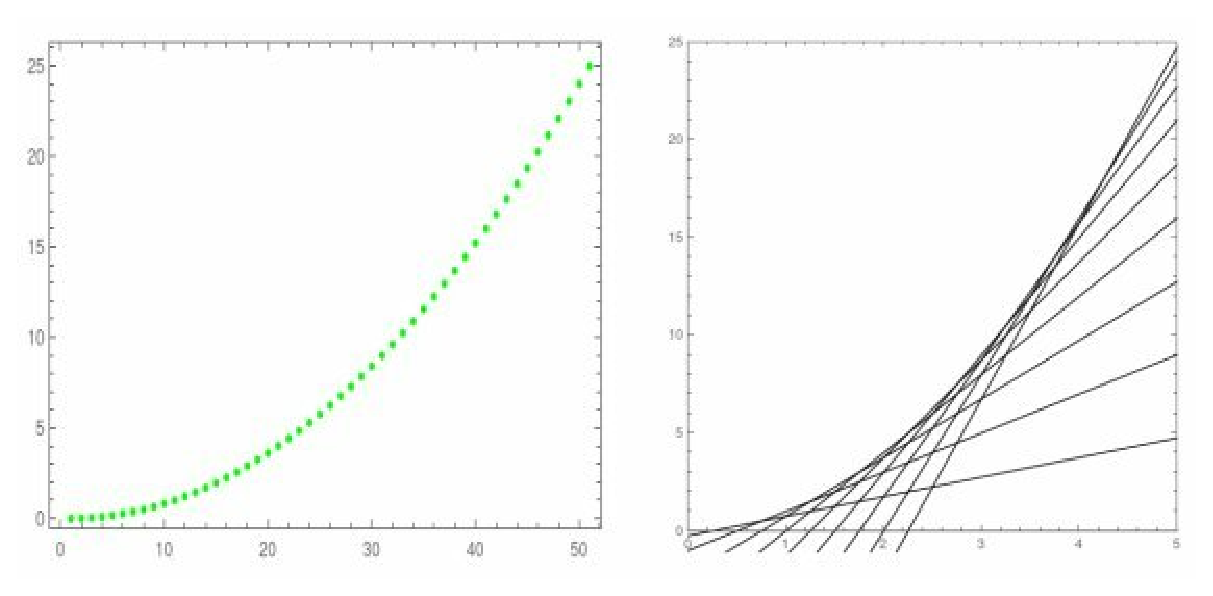
\includegraphics[width=0.75\paperwidth]{question_6/question6.eps} 
\end{center}
\end{figure} 

\subsection{Solution}

Link to the GitHub repository for this question: \href{https://github.com/Xerefic/MM2090-Solutions/tree/master/Final_Assignment/question_6}{GitHub} \footnote{Repo: \url{https://github.com/Xerefic/MM2090-Solutions/tree/master/Final_Assignment/question_6}}

\subsubsection{Approach}
Sampling the given function for 50 points in the range $0 \leq x \leq 100$ and representing the said function using a scatter plot. The transformed function is nothing but the set of lines whose slope correspond to the slope of the tangent at a point $\left(x_i,y_i\right)$ on the polynomial. Using the derivative operation in sagemath, I am computing the slope at a point $x_i$ for $x_i \in f(x)$. At a point $x_i$, the modified function is given by $\frac{y-f(x_i)}{x-x_i}=\frac{\partial f(x)}{\partial x}_{x=x_i}$. 

\subsubsection{Requirements}
Language of choice: sagemath
\begin{lstlisting}[language=bash]
	pip3 install numpy
	pip3 install matplotlib
	pip3 install pandas
\end{lstlisting}

\subsubsection{Images}
The generated plots are for $f(x)=0.01x^2$
NOTE: Please ensure that the function that is to be plotted and operated on is scaled. If the function is not scaled, the output will look congested, and one cannot distinguish the lines in the output.

\begin{figure}[!ht]
	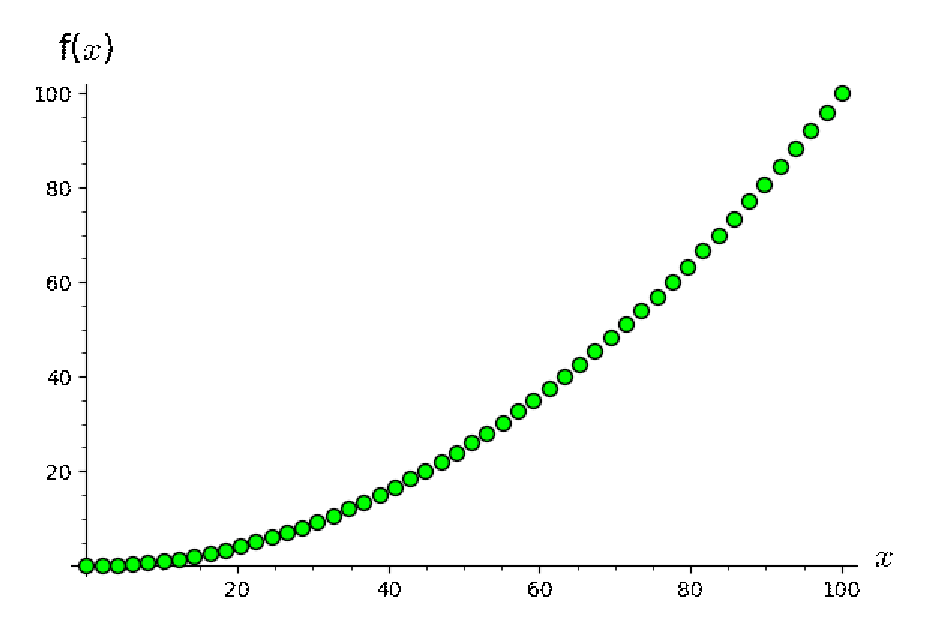
\includegraphics{question_6/Plotted.eps} 
	\caption{Function Plot}
\end{figure} 

\begin{figure}[!ht]
	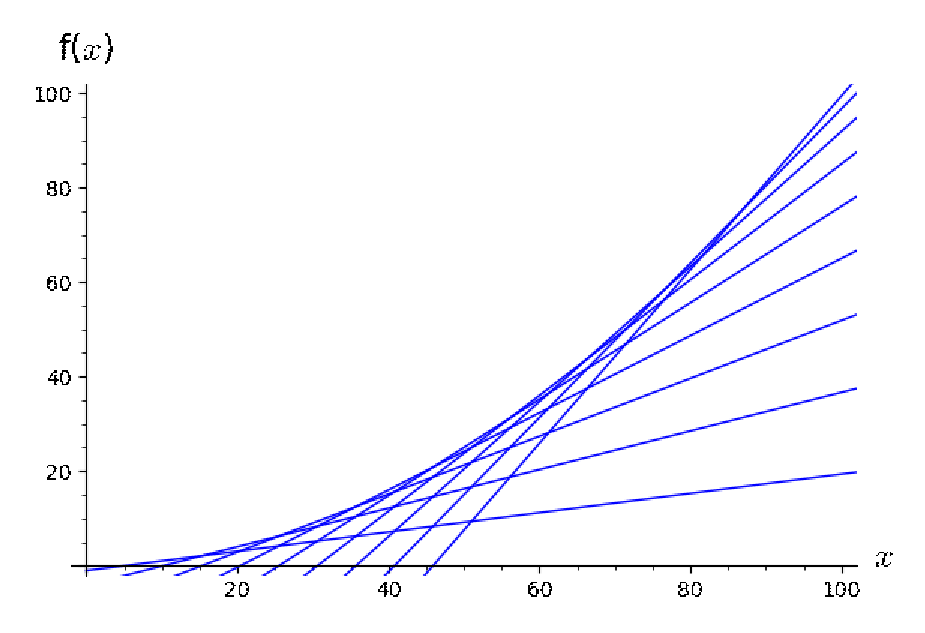
\includegraphics{question_6/Tangents.eps} 
	\caption{Modified Function Plot}
\end{figure} 

\subsubsection{Output}

\begin{table}[!ht]
	\begin{center}
		\begin{tabular}{ | c | c | c | c | }
			\hline
			Coordinates	& Slope & X-Intercept & Y-Intercept \\ \hline
			[0.0, 0.0] & 0.000000 & $\infty$ & 0.000000 \\ \hline
			[10.20, 1.04] & 0.204082 & 5.102041 & -1.041233 \\ \hline
			[20.41, 4.16] & 0.408163 & 10.204082 & -4.164931 \\ \hline
			[30.61, 9.37] & 0.612245 & 15.306122 & -9.371095 \\ \hline
			[40.82, 16.66] & 0.816327 & 20.408163 & -16.659725 \\ \hline
			[51.02, 26.03] & 1.020408 & 25.510204 & -26.030820 \\ \hline
			[61.22, 37.48] & 1.224490 & 30.612245 & -37.484382 \\ \hline
			[71.43, 51.021] & 1.428571 & 35.714286 & -51.020408 \\ \hline
			[81.63, 66.64] & 1.632653 & 40.816327 & -66.638900 \\ \hline
			[91.84, 84.34] & 1.836735 & 45.918367 & -84.339858 \\ \hline
		\end{tabular}
	\end{center}
\caption{Modified Function}
\end{table}

\clearpage
\subsection{Code}
\lstinputlisting{question_6/question6.sage}